\section{Data Preparation}\label{Sec:Data Preparation}

For the analysis explained in this paper data was downloaded for a website independent from airbnb itself. Insideairbnb \citep{insideairbnb} scrapes airbnb to get its data, posts it online for the public to use on own analysis, while also providing some analysis of its own.

The data is divided according to cities and for each there is general information about the city's properties and their availability for the next year. For this analysis not all variables are being kept, the focus is indeed on the ones that might have the most affect on price. Moreover, feature engineering will also be performed to extract even more useful information. More details in subsection \ref{subsec:berlin}.

Since we are dealing with data with coordinates, spatial data is also needed to produce a map of the location. For this purpose further data has been downloaded from the Statistics Office of Berlin-Brandenburg \citep{statberlin:2018} and Geofabrik \citep{geofabrik:2018} and further processed, as explained in subsections \ref{subsec:berlin} and \ref{subsec:vbb}.

To handle data will be make use of functions from the different packages in the \texttt{tidyverse}, which allows for easy manipulation of the data and flexible plotting, see \cite{ross2017declutter}. For spatial data the package \texttt{sf} has been chosen, since it works well with the \texttt{tidyverse} packages and for all the other reasons listed in \cite{pebesma2018simple}.


\subsection{Berlin neighbourhoods and districts}\label{subsec:berlin}

Berlin consists of 96 neighbourhoods (Ortsteile), which are grouped into 12 districts (Bezirke). The data downloaded from  \cite{statberlin:2018} contain one polygon for each neighbourhood and additional information about them, out of which we only kept the district.

The polygons have been extracted from the relative shapefile with the function \texttt{st\_read} from the \texttt{sf} package. For the neighbourhoods we simply rename the variables and keep the ones of interest.

\lstinputlisting[language=R, firstline=19, lastline=28, firstnumber=1, escapechar=|, caption={|\textbf{\href{https://github.com/silvia-ventoruzzo/SPL-WISE-2018/blob/master/SPL_Berlin_Districts_Neighbourhoods/berlin_districts_neighbourhoods.R}{berlin\_districts\_neighbourhoods.R}}|}]{../SPL_Berlin_Districts_Neighbourhoods/berlin_districts_neighbourhoods.R}

However, one of the neighbourhoods, Buckow, is composed of two separate polygons, which we therefore need to unite according to the neighbourhoods' names. Thanks to the flexibility of the \texttt{sf} objects, this is done simply with a \texttt{summarize} from the package \texttt{dyplr}.

\lstinputlisting[language=R, firstline=31, lastline=33, firstnumber=11, escapechar=|, caption={|\textbf{\href{https://github.com/silvia-ventoruzzo/SPL-WISE-2018/blob/master/SPL_Berlin_Districts_Neighbourhoods/berlin_districts_neighbourhoods.R}{berlin\_districts\_neighbourhoods.R}}|}]{../SPL_Berlin_Districts_Neighbourhoods/berlin_districts_neighbourhoods.R}

For the districts we perform the same procedure as above, but this time we unite the polygons only by their district, which are represented here by the group variable.

\lstinputlisting[language=R, firstline=36, lastline=39, firstnumber=19, escapechar=|, caption={|\textbf{\href{https://github.com/silvia-ventoruzzo/SPL-WISE-2018/blob/master/SPL_Berlin_Districts_Neighbourhoods/berlin_districts_neighbourhoods.R}{berlin\_districts\_neighbourhoods.R}}|}]{../SPL_Berlin_Districts_Neighbourhoods/berlin_districts_neighbourhoods.R}

The produced polygons can be used to map Berlin using \texttt{ggplot2} or \texttt{leaflet}, as shown in figure \ref{figure:berlin_map}. \texttt{leaflet} is more flexible and more suitable for plotting spatial data. Therefore, this package will be used for now on for mapping polygons and coordinate points.


\begin{figure}[H]
\centering
\subfloat[With \texttt{leaflet}]{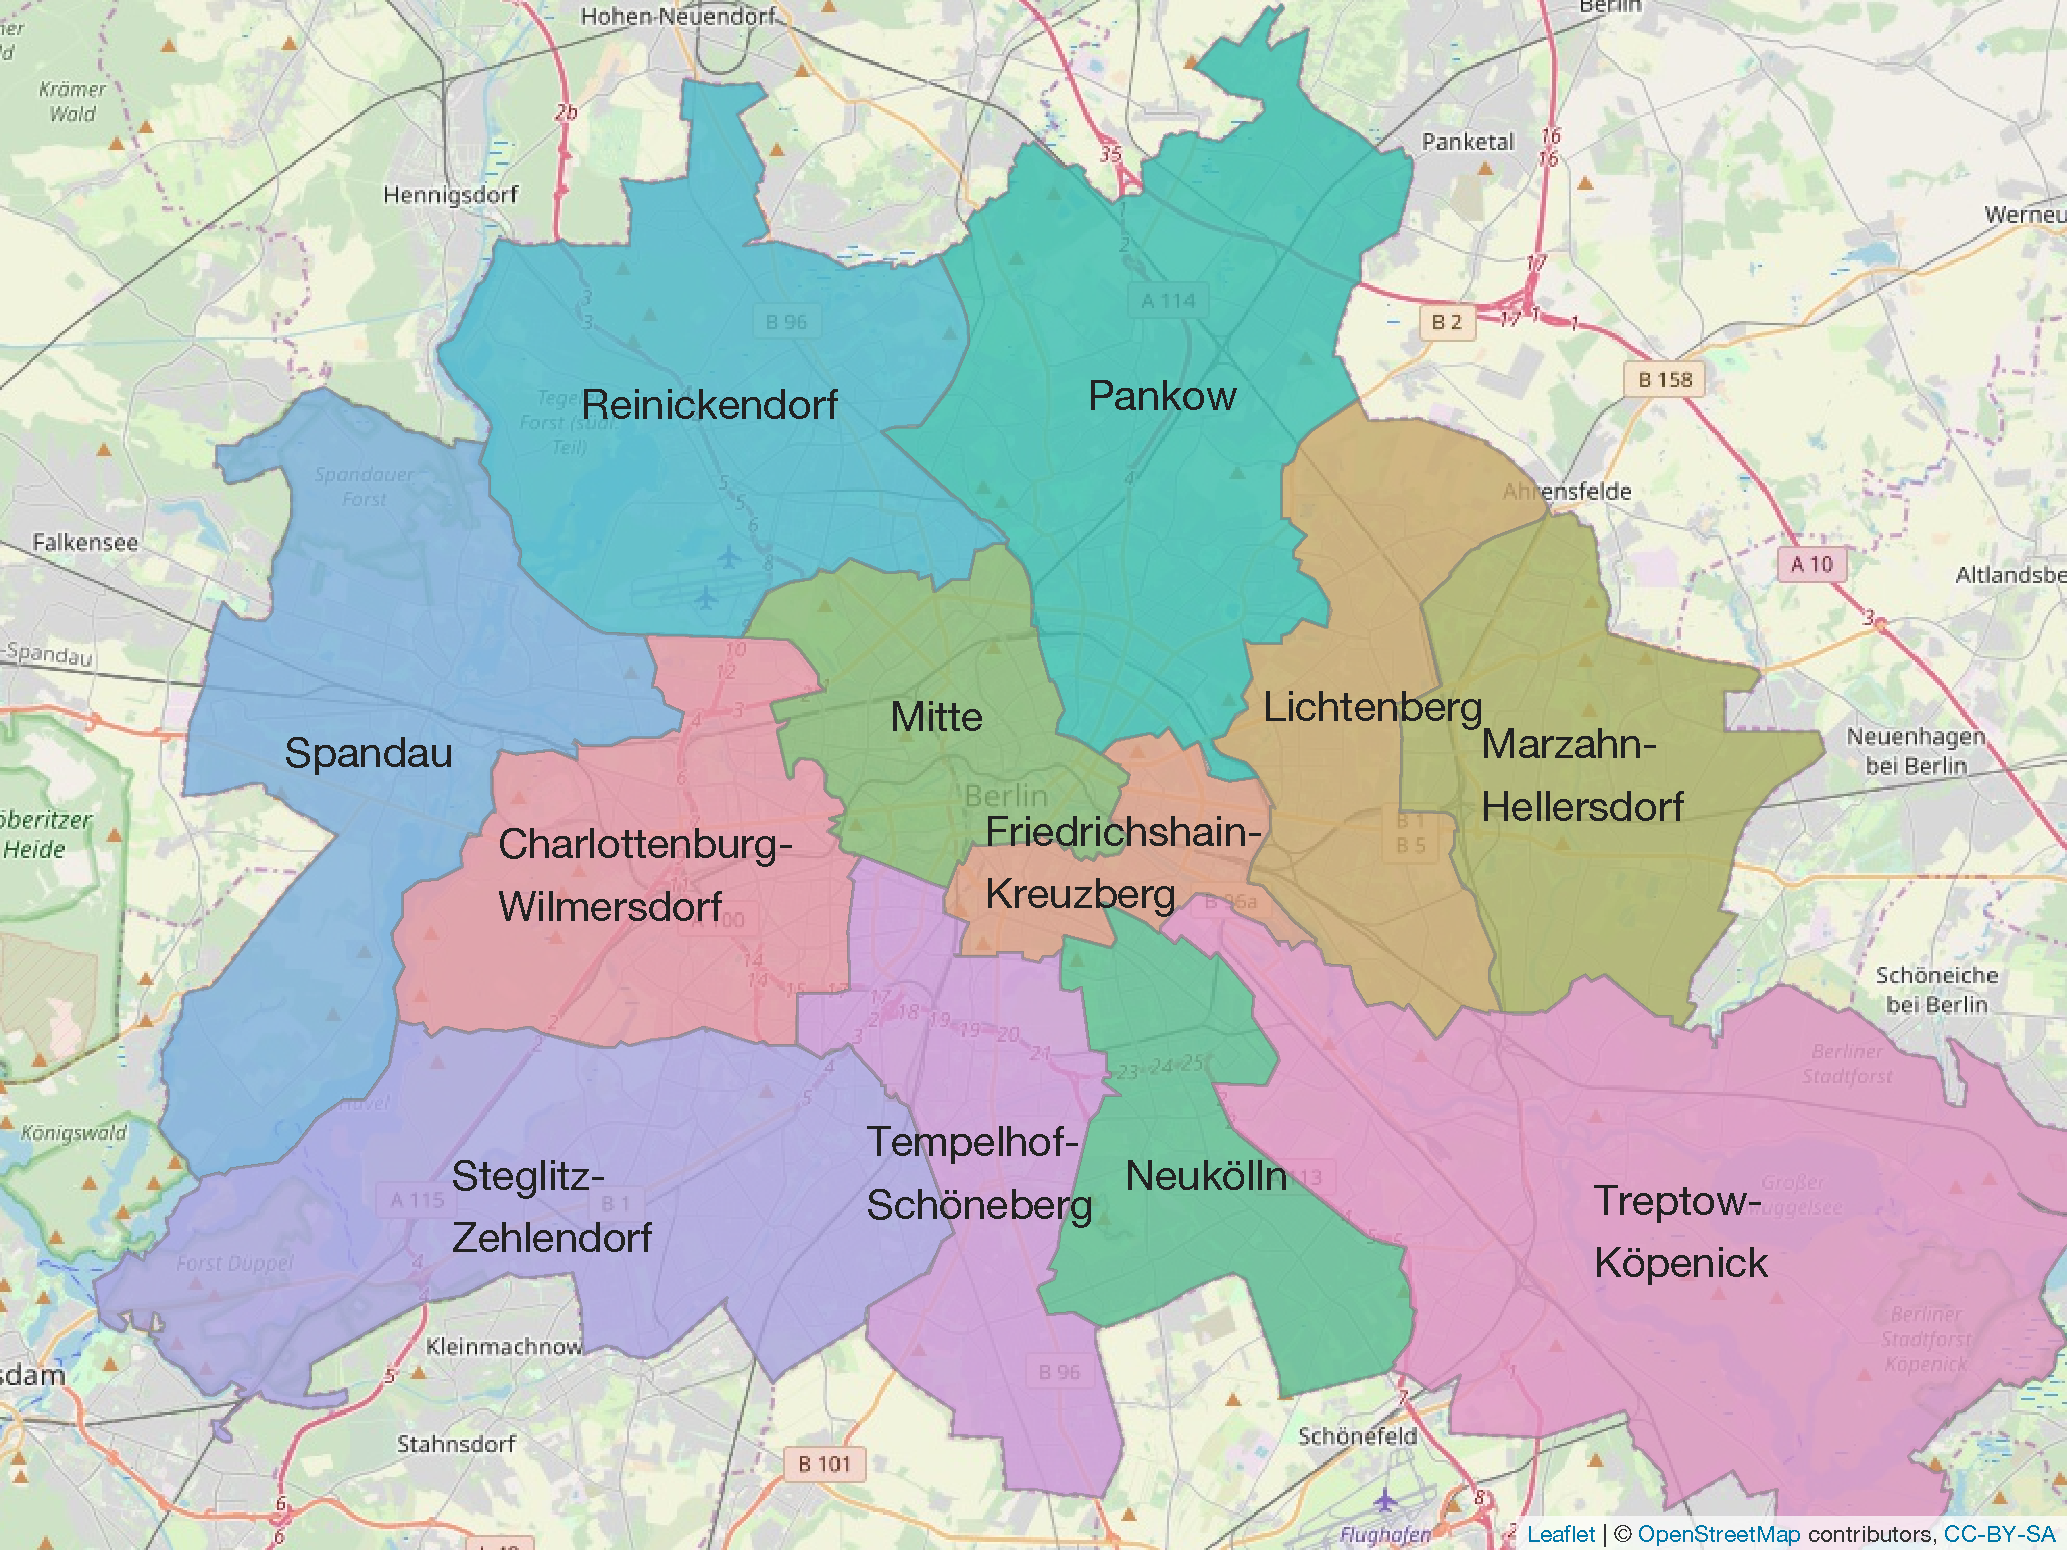
\includegraphics[width=0.4\textwidth]{berlin_district_leaflet.pdf}}
\subfloat[With \texttt{ggplot2}]{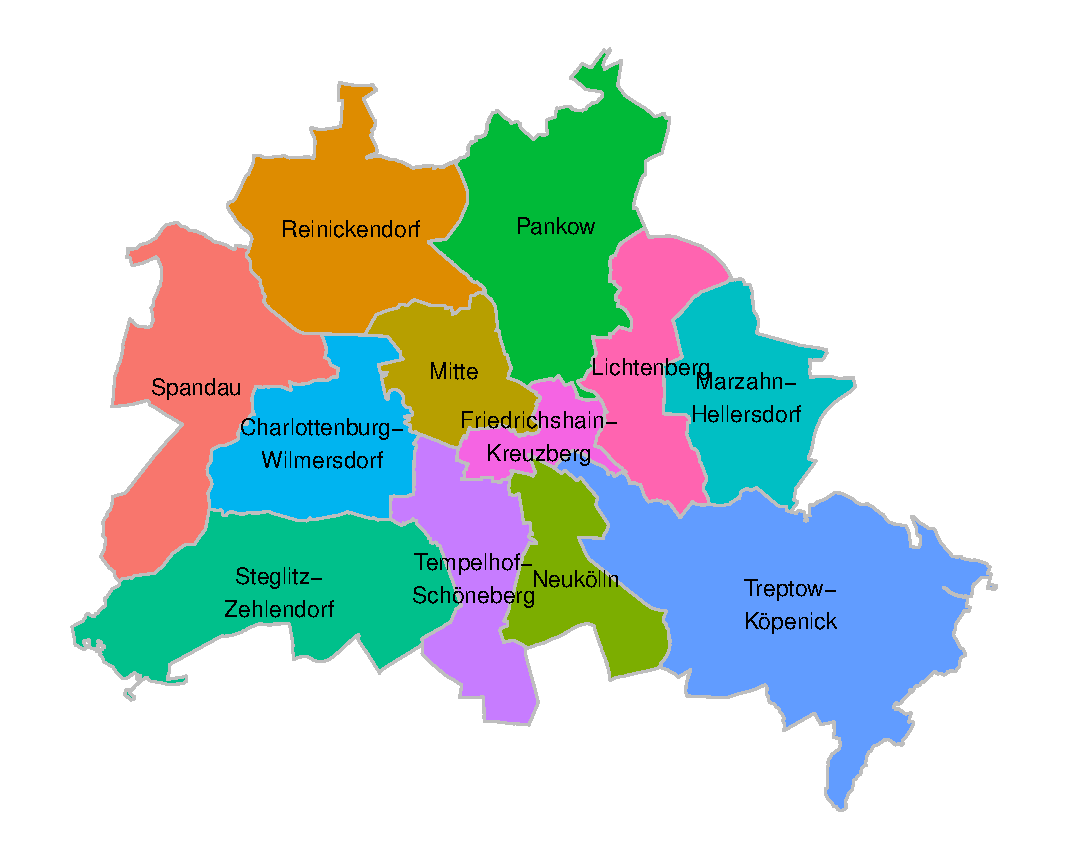
\includegraphics[width=0.4\textwidth]{berlin_district_ggplot.pdf}}
\caption{Maps of the Berlin Districts \protect
\includegraphics[scale=0.05]{qletlogo.pdf} {\href{https://github.com/silvia-ventoruzzo/SPL-WISE-2018/blob/master/Berlin_Districts_Neighbourhoods/berlin_districts_neighbourhoods_maps.R}{berlin\_districts\_neighbourhoods\_maps.R}}}
\centering
\label{figure:berlin_map}
\end{figure}

\subsection{Berlin VBB Zones}\label{subsec:vbb}

The VBB (Verkehrsverbund Berlin-Brandenburg) is "the public transport authority covering the federal states of Berlin and Brandenburg" \citep{vbb:2019}. The city of Berlin, in particular, is divided in two fare areas: A, covering the center of Berlin up to the circular line (Ringbahn), and B, from the Ringbahn to the border with Brandenburg. After that there is also the area C, which however will not be covered here since we only consider the city of Berlin.

\begin{figure}[H]
\begin{center}
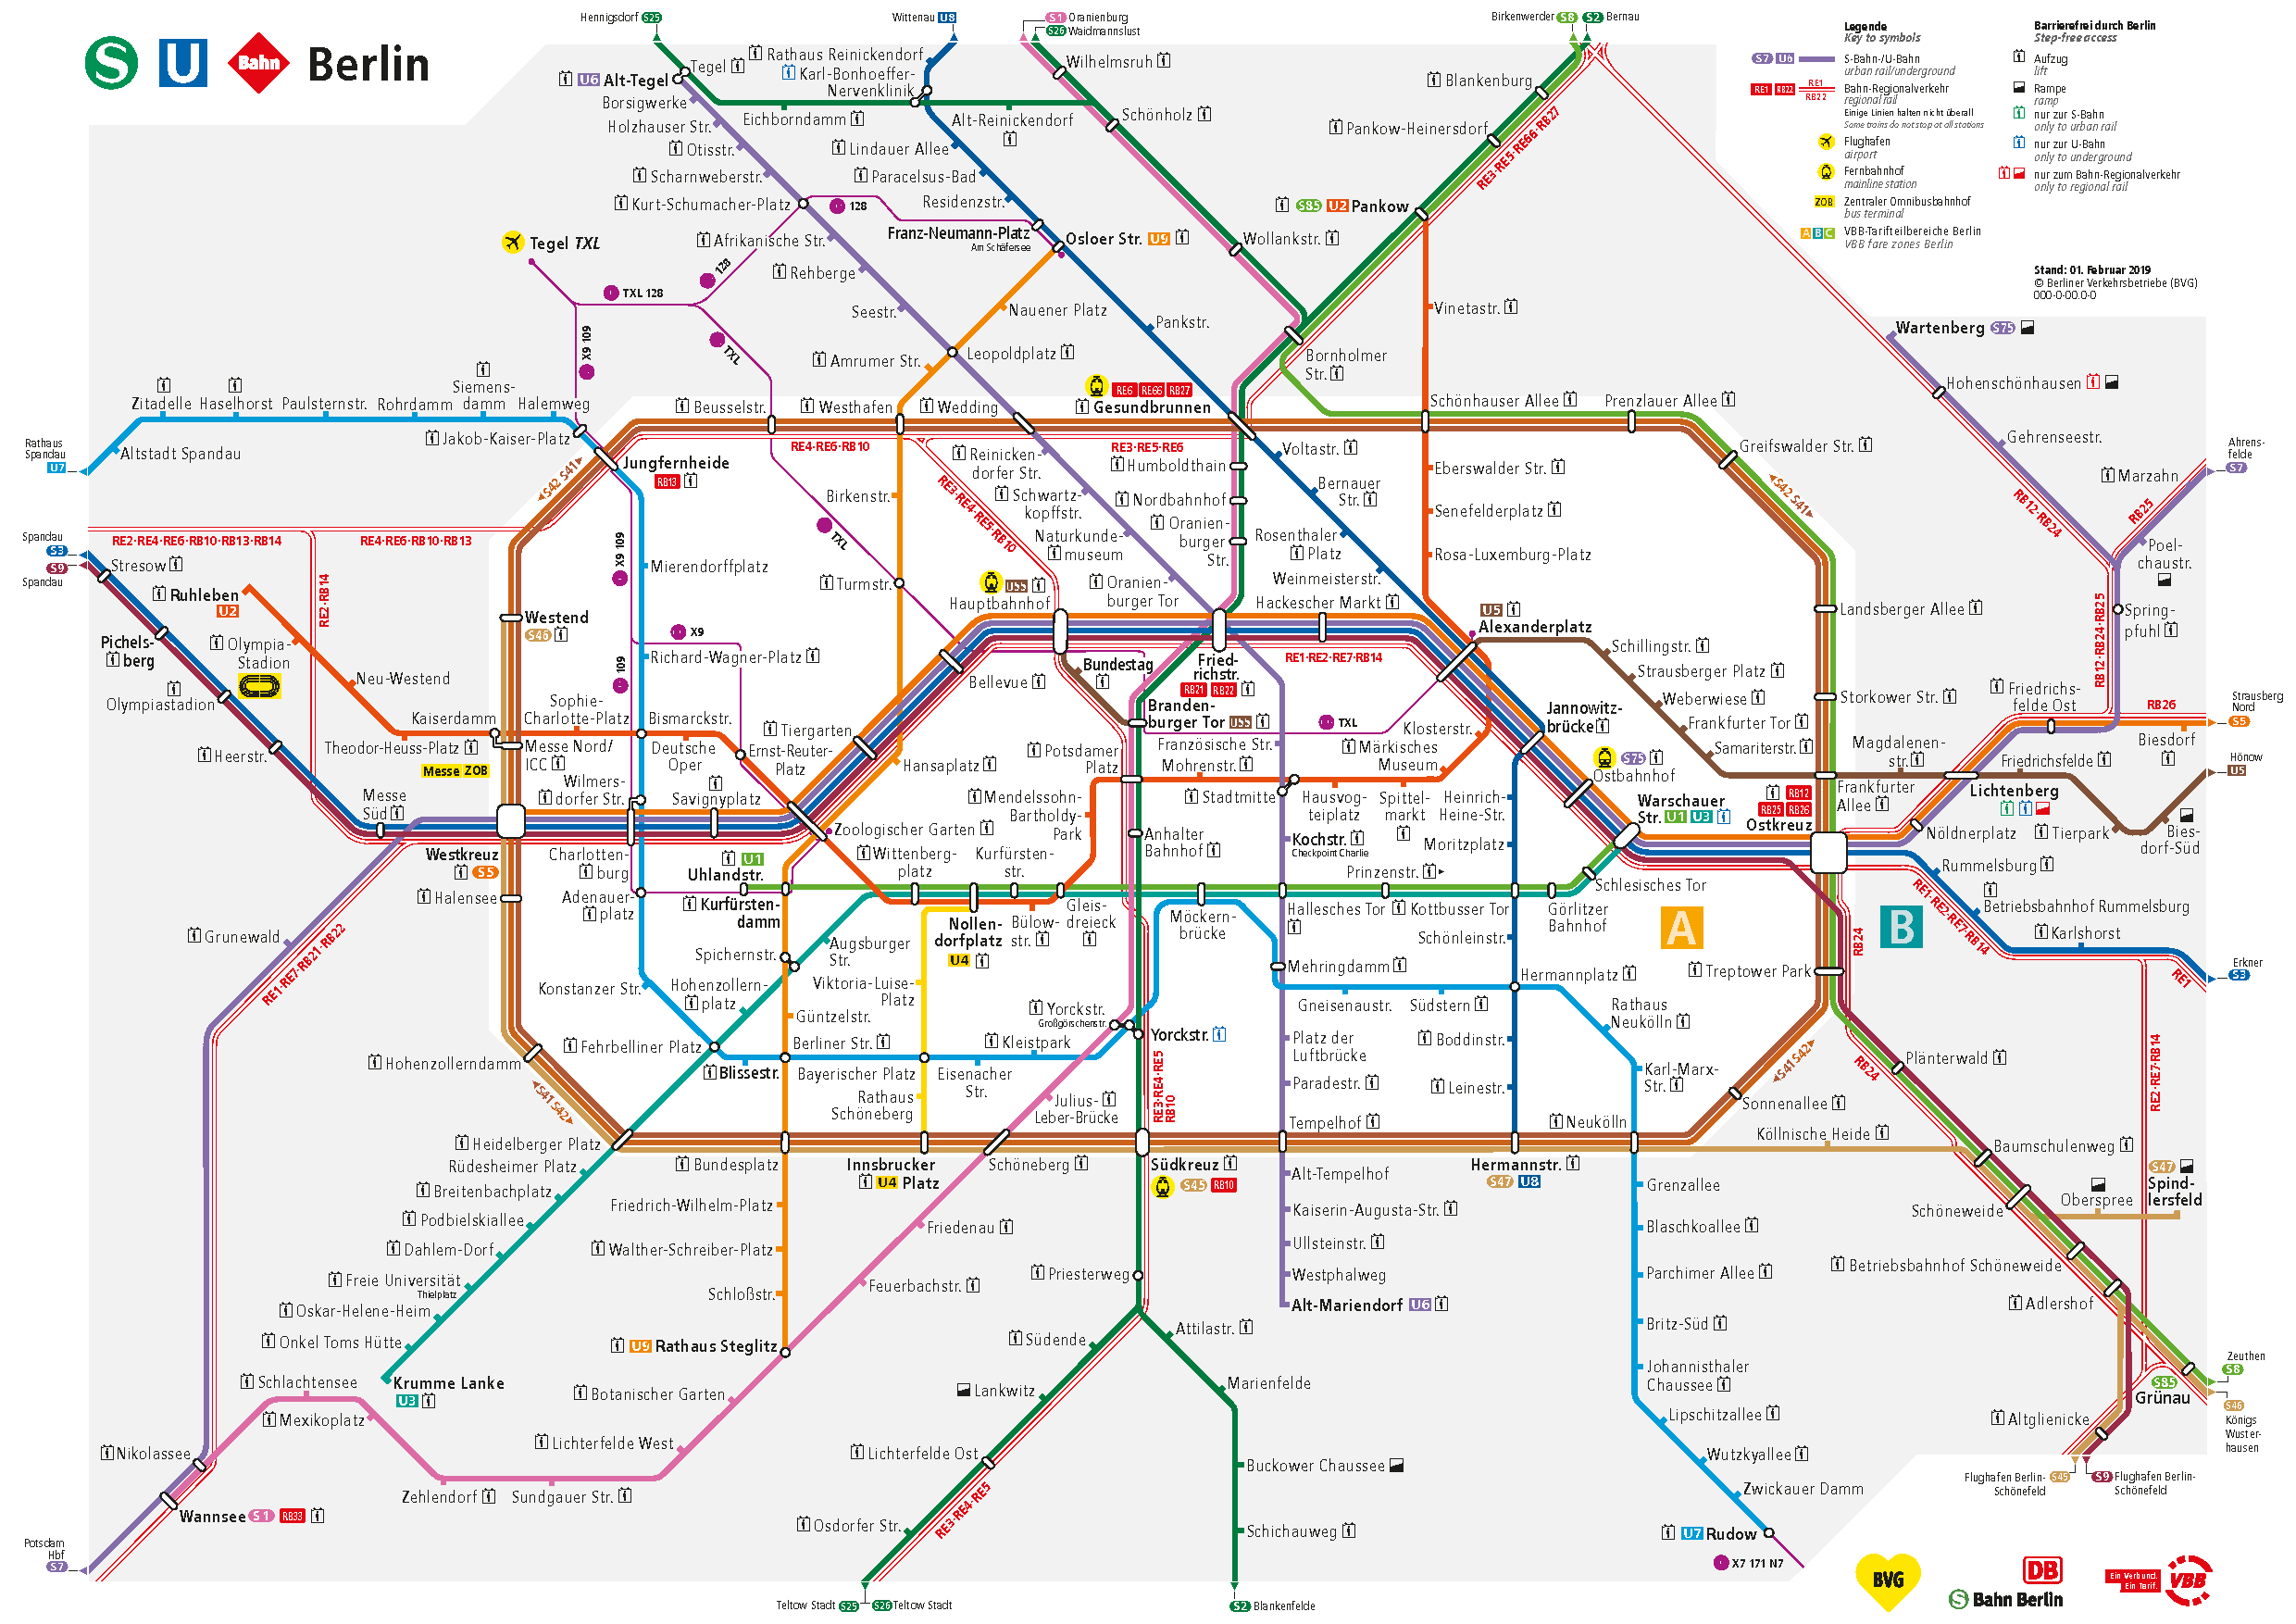
\includegraphics[width=0.8\textwidth, keepaspectratio]{S_und_U-Bahnnetz_mit_Regionalbahn_Innenstadt.pdf} \\
\caption{Network Map of Berlin Areas A and B (Source: \cite{vbb:2019})}
\end{center}
\end{figure}

We tried to replicate these areas by also making use of the spatial points of the Berlin stations.

First of all, we need to create the polygon for area A, which is done by joining the points in the circular line and transforming this into a polygon.

Unfortunately the shapefile with the stations did not contain information about the line to which these stations correspond. Therefore we needed to filter the stations manually with the ones belonging to the circular line. This vector also contains the information in which order the points will be connected. You can notice that the first and last station are the same since the polygon needs to close.

\lstinputlisting[language=R, firstline=29, lastline=40, firstnumber=1, escapechar=|, caption={|\textbf{\href{https://github.com/silvia-ventoruzzo/SPL-WISE-2018/blob/master/SPL_Berlin_VBB_Zones/berlin_vbb_zones.R}{berlin\_vbb\_zones.R}}|}]{../SPL_Berlin_VBB_Zones/berlin_vbb_zones.R}

Since some stations appear multiple times, we firstly filter railway stations, which include both subway and lightrail, and then we calculate the middle point for each station among the ones having the same name. We then join this with the dataframe containing the names of the stations in the circular line, thus filtering the stations to the ones we are interested in. After performing some preparation steps, the function \texttt{st\_polygon} from the \texttt{sf} package was used to create a polygon out of a list of points.

\lstinputlisting[language=R, firstline=43, lastline=59, firstnumber=13, escapechar=|, caption={|\textbf{\href{https://github.com/silvia-ventoruzzo/SPL-WISE-2018/blob/master/SPL_Berlin_VBB_Zones/berlin_vbb_zones.R}{berlin\_vbb\_zones.R}}|}]{../SPL_Berlin_VBB_Zones/berlin_vbb_zones.R}

Second af all, in order to create the polygon for zone B, we need to produce the  polygon for entire Berlin. This is done with a procedure already explained in subsection \ref{subsec:berlin}. In this case we don't perform any grouping, thus uniting all neighbourhoods.

\lstinputlisting[language=R, firstline=62, lastline=63, firstnumber=31, escapechar=|, caption={|\textbf{\href{https://github.com/silvia-ventoruzzo/SPL-WISE-2018/blob/master/SPL_Berlin_VBB_Zones/berlin_vbb_zones.R}{berlin\_vbb\_zones.R}}|}]{../SPL_Berlin_VBB_Zones/berlin_vbb_zones.R}

Finally, we bind the two objects by row and calculate their intersections thanks to the function \texttt{st\_intersection} from the package \texttt{sf}. We then define the area names according to how many times the two previous polygons intersect:
	\begin{itemize}
    		\item Area A: where polygons intersect (n. overlaps > 1)
    		\item Area B: where polygons do not intersect (n. overlaps $\leq$ 1)
    \end{itemize}

\lstinputlisting[language=R, firstline=66, lastline=71, firstnumber=34, escapechar=|, caption={|\textbf{\href{https://github.com/silvia-ventoruzzo/SPL-WISE-2018/blob/master/SPL_Berlin_VBB_Zones/berlin_vbb_zones.R}{berlin\_vbb\_zones.R}}|}]{../SPL_Berlin_VBB_Zones/berlin_vbb_zones.R}

\iffalse
In this code the custom-function \texttt{points\_midpoint} was used to calculate the middle point among many. It extracts the coordinates of the points thanks to \texttt{st\_coordinates} and then calculates the mean of latitude and longitude.

\lstinputlisting[language=R, firstline=2, escapechar=|, caption={|\textbf{\href{https://github.com/silvia-ventoruzzo/SPL-WISE-2018/blob/master//Helpers/points_midpoint.R}{points\_midpoint.R}}|}]{../Berlin_VBB_Zones/Helpers/points_midpoint.R}
\fi

As in subsection \ref{subsec:berlin} the \texttt{sf} object can be used to map the VBB zones using \texttt{leaflet} or \texttt{ggplot2}.

\begin{figure}[H]
\centering
\subfloat[With \texttt{leaflet}]{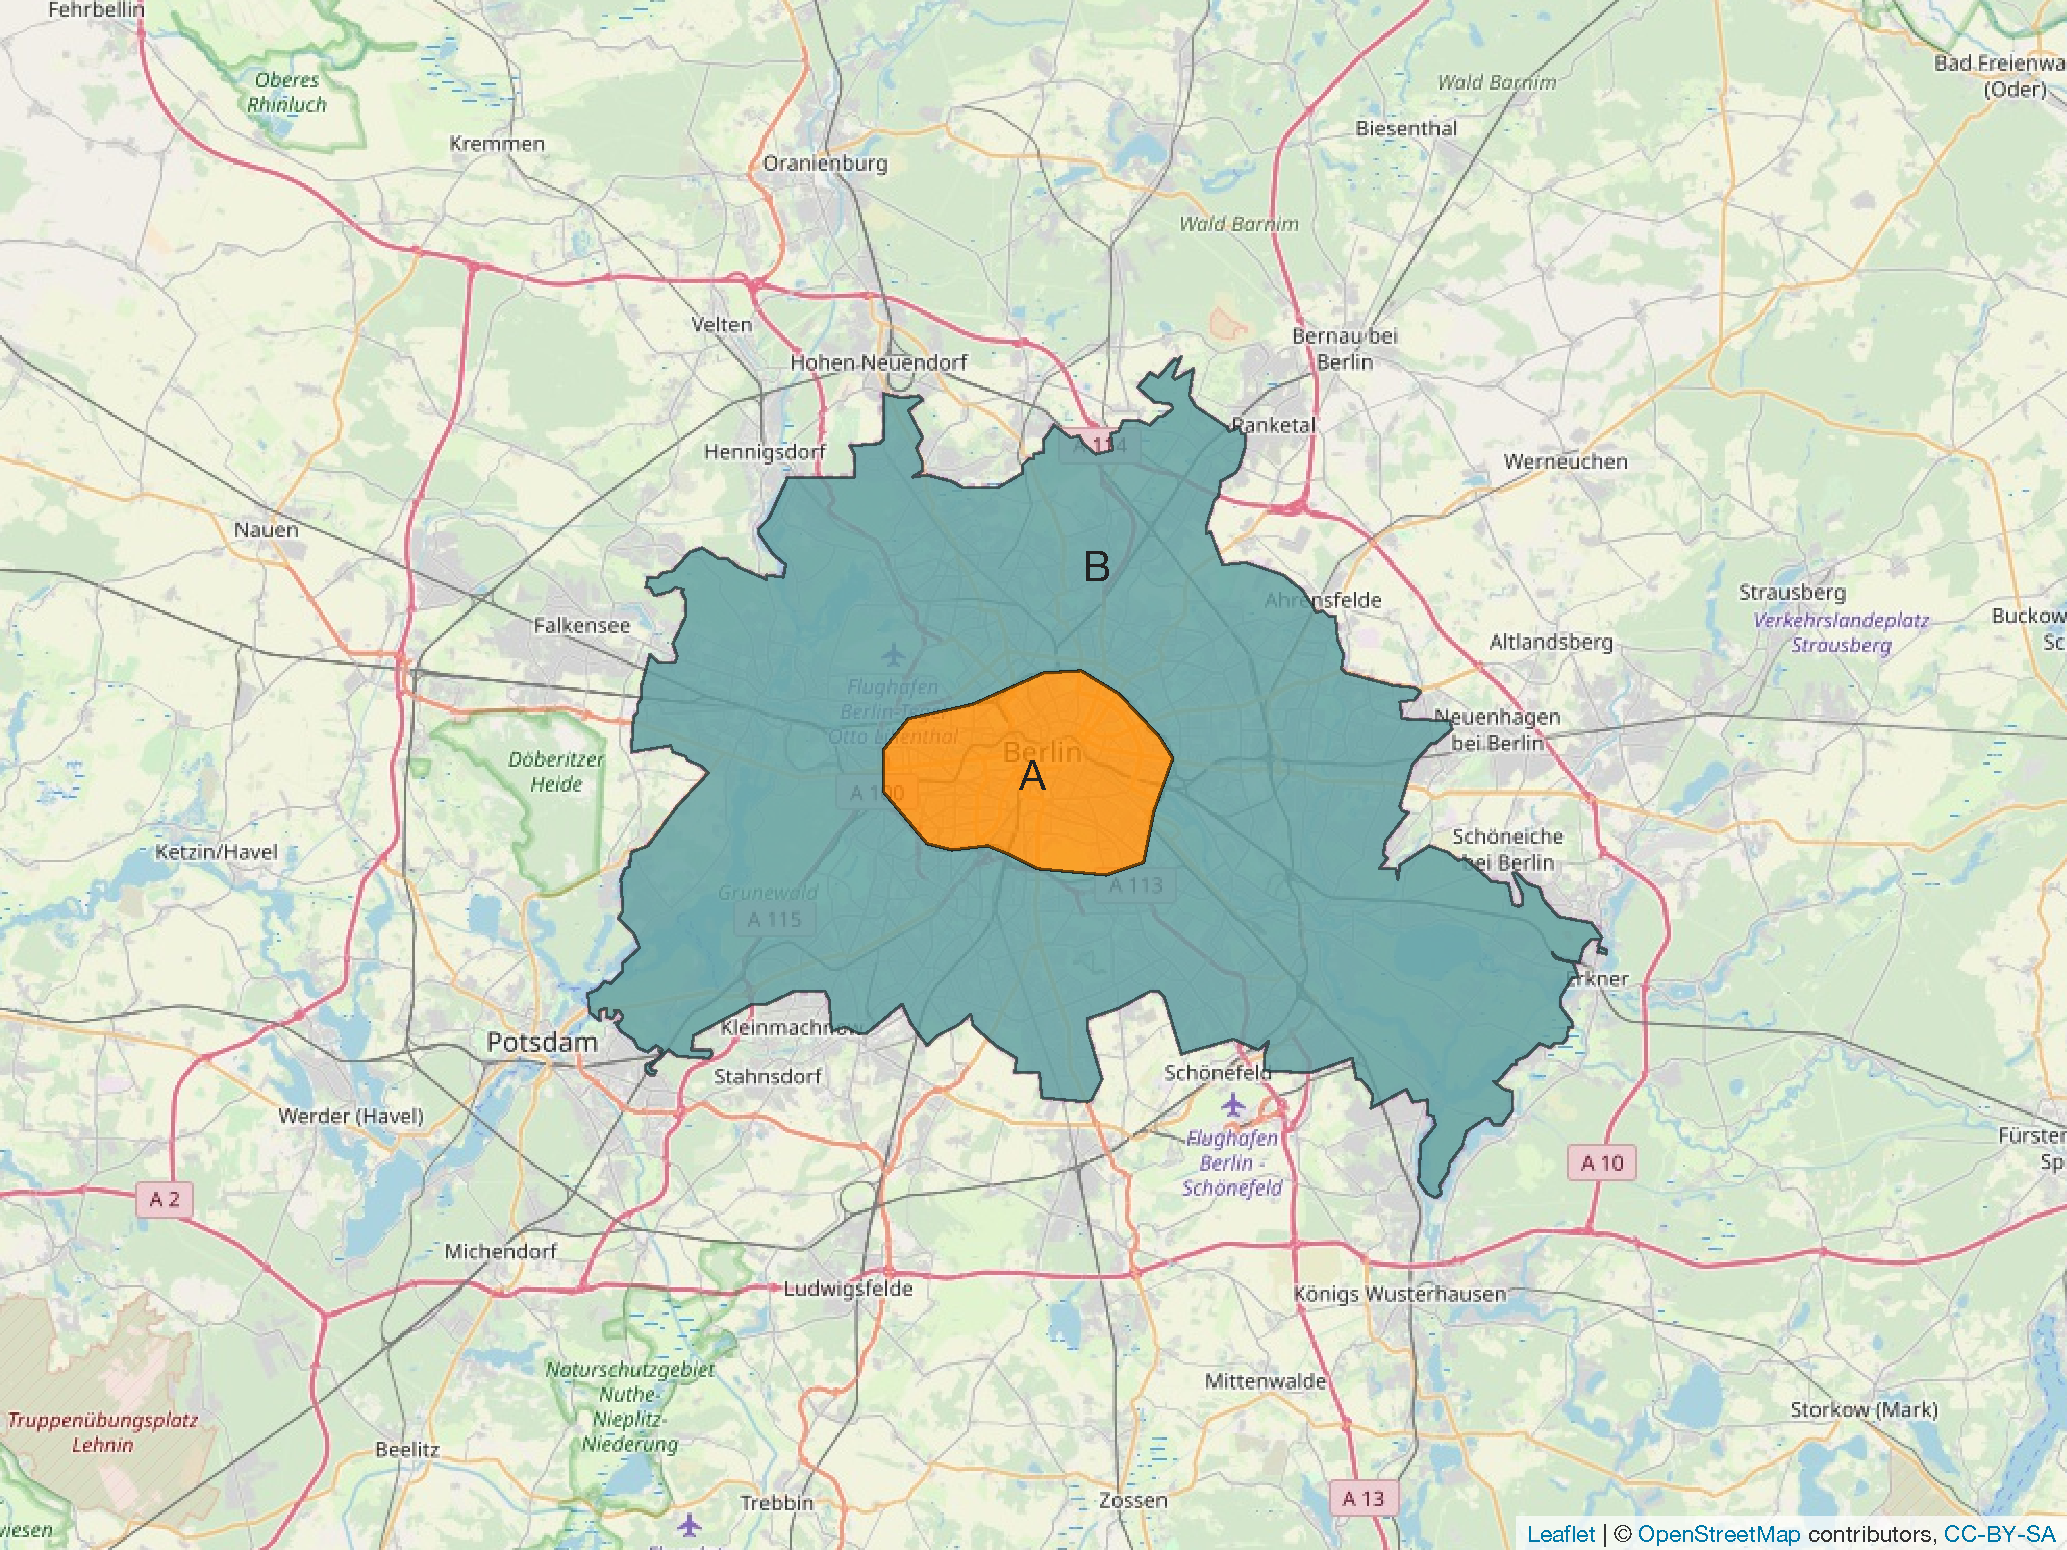
\includegraphics[width=0.4\textwidth]{berlin_vbb_zones_leaflet.pdf}}
\subfloat[With \texttt{ggplot}]{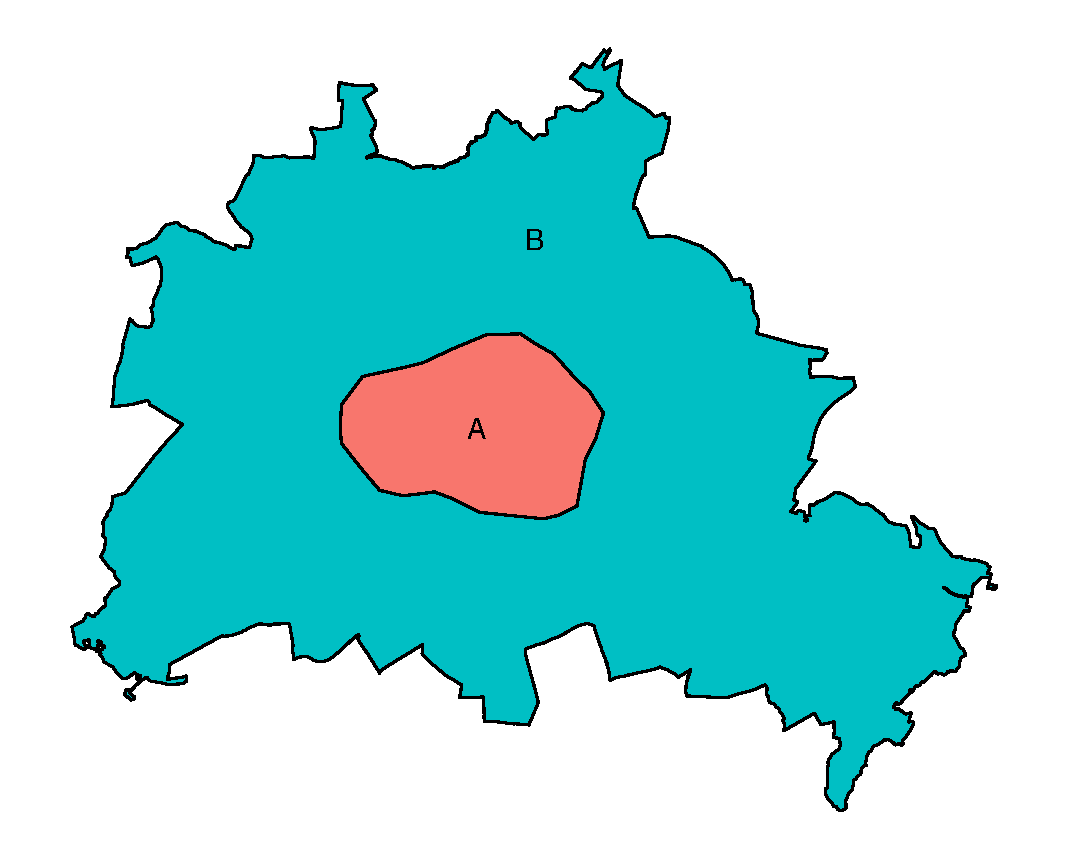
\includegraphics[width=0.4\textwidth]{berlin_vbb_zones_ggplot.pdf}}
\caption{Maps of the Berlin VBB Zones \protect
\includegraphics[scale=0.05]{qletlogo.pdf} {\href{https://github.com/silvia-ventoruzzo/SPL-WISE-2018/blob/master/Berlin_VBB_Zones/berlin_vbb_zones_maps.R}{berlin\_vbb\_zones\_maps.R}}}
\centering
\end{figure}

\subsection{Airbnb listings' attributes}\label{subsec:airbnb}

The first part of cleaning the airbnb data consists in joining the two datasets containing general information according to their common variables and correcting some string values. Secondly, we proceed in checking for missing values and deriving that information from other correlated variables. Thirdly, we move on to feature engineering.

We firstly derive the areas where the properties are located thanks to the spatial polygons created before and the function \texttt{point\_in\_polygons}.
This function loops through the polygons in the \texttt{sf} object and check which points are contained in which polygons. In the end it writes the id associated to the polygon, in our case the area id, in the summary column, which can be named as preferred.

\lstinputlisting[language=R, firstline=2, escapechar=|, caption={|\textbf{\href{https://github.com/silvia-ventoruzzo/SPL-WISE-2018/blob/master/Helpers/point_in_polygons.R}{point\_in\_polygons.R}}|}]{../Helpers/point_in_polygons.R}

Secondly, for railway stations and tourist attractions we calculate the amount inside a range and the distance to the nearest point using the function \texttt{distance\_count}. In particular, the following parameters will be used:

\begin{itemize}

    \item Railway stations: distance = 1000 (1 km)

    \item (Top 10) attractions: distance = 2000 (2 km)
    
\end{itemize}

This function firstly calculates the distance between all properties and all reference points using the Haversine Formula, which "gives  minimum  distance  between  any  two  points  on  spherical body by using latitude and longitude" \citep{ingole2013landmark} according to the following formula:

\begin{equation}
d = 2r \arcsin \Bigg(\sqrt{\sin^2\Big(\frac{\phi_2 - \phi_1}{2}\Big) + \cos(\phi_2)\cos(\phi_1)\sin^2\Big(\frac{\psi_2 - \psi_1}{2}\Big)}\Bigg)
\end{equation}

where $\phi$ corresponds to the latitude and $\psi$ to the longitude of the two points.

Then it calculates how many reference points are within the set distance and how much is the distance to the nearest reference point. Finally this information is joined into the main dataframe.

\lstinputlisting[language=R, firstline=3, escapechar=|, caption={|\textbf{\href{https://github.com/silvia-ventoruzzo/SPL-WISE-2018/blob/master/Helpers/distance_count.R}{distance\_count.R}}|}]{../Helpers/distance_count.R}

In the end we use the calendar dataframe to calculate availability of each property in the different seasons.

\lstinputlisting[language=R, firstline=192, lastline=208, caption={|\textbf{\href{https://github.com/silvia-ventoruzzo/SPL-WISE-2018/blob/master/data_preparation.R}{data\_preparation.R}}|}]{../data_preparation.R}